\chapter{System Overview}

\section{System Features}
The system will use rule based information extraction technique to parse the job description and resume, and get information such as skill, specialties and background. These information will be used to create the model of job description and job seeker.  Ontology will be used to construct the knowledge base, which will include the taxonomy and rules, to support resume-job matching.

The model of candidates will include their specialties, working experience and education background, all the them should be extracted from the resumes. The job model will be extracted from job description, the information will include: company name, location, job title, education requirement, skill requirements and working experiences etc. When a job seeker searches the jobs by his resume, the system will calculate the similarity between the candidate model and the job models, give every job model a similarity score.

In the initial phase I will only focus on the positions of IT job, because IT jobs have a special character,  skill set oriented, which means the person that the company want to hire must have some special skills and knowledge, like some programming languages, databases or software etc.

User��s personal preference should be considered as well. In the previous user survey, some factors will impact a lot on the user��s expectation of good jobs, such factors include: location, the reputation of the company, the salary etc. These factors will be treated as weight factors in the job matching algorithm.

\section{System Architecture}

Figure ~\ref{fig:Pipeline} shows the architecture of the whole system, which include such modules:

\begin{enumerate}
    \item The web scrawler could search and download all new IT job opening web pages  from indeed.com everyday.
    \item Job parser could parse the job opening web page, extract the information and create the job model.
    \item Resume Parser is much like the Job parser, it will parse the resume and create the candidate model.
    \item All the job models will be stored in the Job Description database.
    \item When user make a query request, the ontology matcher will calculate the matching score of each job, return the jobs ranked by their scores.
\end{enumerate}

\begin{figure}[htbp]
  \centering
  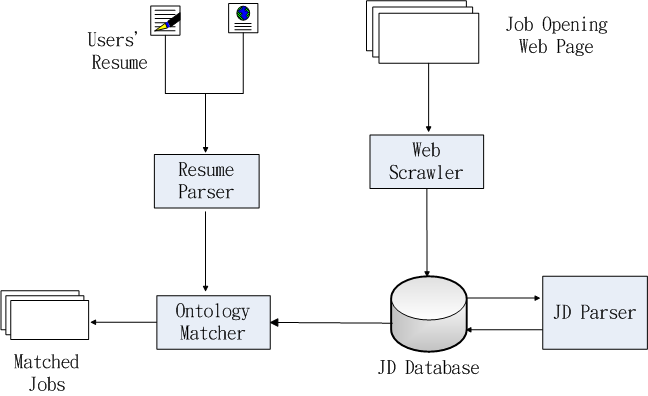
\includegraphics[scale=0.5]{images/arch.png}
  \caption{System Architecture}
  \label{fig:arch}
\end{figure}

The system should include such features:

\begin{enumerate}
    \item User could import his resume in different format, like txt, doc and pdf.
    \item User could search jobs by his resume. The search result will be sorted by the matching scores.
    \item User could set their searching preference, like location, company type, reputation, salary level, etc.
    \item The system should be able to change the parameters of the matching algorithm adaptively according to the record of user's preference
    \item The user could set multiple searching agents, each one of which is a composition of different preferences, like one for remote location with high salary, another for local company with low salary.
\end{enumerate}
